%----------------------------------------------------------%
% !TEX outputDirectory = build

\documentclass[reqno,a4paper,12pt]{amsart}
\def\thmcolor{black!10}
\def\defcolor{black!10}
\input{header.tex}

\usepackage{tikz}
\usetikzlibrary{patterns}
\usepackage{algorithm}
\usepackage[noend]{algpseudocode}

% Temporary nonsense
\usepackage{pgfplots}
\pgfplotsset{compat=1.15,width=10cm,height=10cm}

%----------------------------------------------------------%
%% Document specific definitions

%% Comments
\newcommand{\victor}[1]{\textcolor{magenta}{\textbf{[#1]}}}
\newcommand{\afonso}[1]{\textcolor{red}{\textbf{[#1]}}}
\newcommand{\roberto}[1]{\textcolor{blue}{\textbf{[#1]}}}
\newcommand{\felipe}[1]{\textcolor{orange}{\textbf{[#1]}}}

%----------------------------------------------------------%

\begin{document}

\title{O número de conjuntos de Sidon forte}

\author{Felipe Guimarães}
\author{Roberto Parente}
\author{Afonso Sant'Anna}
\author{Victor Souza}

%----------------------------------------------------------%

\begin{abstract}
Rascunho em português.
\end{abstract}

\maketitle

%----------------------------------------------------------%

\section{Introdução}
\label{sec:intro}

Um subconjunto $A \subseteq \ZZ$ é dito um conjunto de \emph{Sidon $k$-forte} se para quaisquer $x, y, z, w \in A$ com $x < z \leq w < y$, vale que $\abs{x + y - z - w} \geq k$.
Um conjunto de Sidon é um conjunto $1$-forte.
Denote por $\cS_k(A)$ a família de todos os subconjuntos $S \subseteq A$ que são Sidon $k$-forte, isso é,
\begin{equation*}
    \cS_k(A) \defined \set[\big]{S \subseteq A \st \text{$A$ é um conjunto de Sidon $k$-forte}}.
\end{equation*}

O nosso objetivo é provar um resultado como o seguinte.

%--------------------------------------%
\begin{theorem}
\label{theoprincp}
Existem constantes $0 < c \leq C$ tais que o número de subconjuntos de $[n]$ que são de Sidon $k$-forte satisfaz
\begin{equation*}
    2^{(1- o(1) )c F(n,k)} \leq \card[\big]{\cS_k([n])} \leq 2^{(1+ o(1))C F(n,k)}
\end{equation*}
quando $n \to \infty$ e $k$ satisfaz certas condições a serem determinadas \victor{Por exemplo, $k$ não pode ser muito próximo de $n$.}.
A função $F(n,k)$ é o que precisamos determinar, por exemplo, é possível que $F(n,k) = \log(1 + k)\sqrt{n/k}$ seja a função correta.
\end{theorem}
%--------------------------------------%

Para o limite inferior, a ideia de prova será baseada na prova do Teorema de Saxton-Thomason que mostra que o limite inferior para o número de conjuntos de Sidon é $2^{1.16\sqrt{n}}$. Usando a notação acima, podemos enunciar o Teorema de Saxton-Thomason da seguinte forma:

\begin{theorem}[Saxton-Thomasson]
    Seja $n \in \mathbb N$, vale que $\mathcal{S}_1([n])\geq 2^{1.16\sqrt{n}}$.
\end{theorem}
\begin{proof}

\label{ProofSax}
Seja $t\geq 1$ um inteiro e defina \[m \coloneqq \Big\lfloor\frac{n}{t}\Big\rfloor.\]
Seja $A \subseteq \mathbb Z_m$ um conjunto de Sidon com cardinalidade máxima. Por resultados anteriores, existe $A$ tal que \[ s\coloneqq |A|=(1+o(1))\sqrt{m}.\]

Para cada função \[f : \; A \to \{\bot,0,1,...,t-1\},\]
defina \[A_f\coloneqq \{\,a+\delta m: \; a\in A,\; f(a)=\delta \in \{0,\dots,t-1\}\,\} \subseteq [n].\]
Onde $f(a)= \bot$ significa "não escolher $a$" e $f(a)=\delta \in \{0,\dots, t-1\}$ significa que incluímos $a$ no bloco de índice $\delta.$
Observe que para cada $a \in A$ existem $t+1$ escolhas independentes, logo o número de funções é $(t+1)^s.$

Queremos mostrar agora que para qualquer $f$, o conjunto $A_f$ é um conjunto de Sidon em $[n]$. Sejam
\[
x,y,z,w\in A_f
\]
com
\[
x+y=z+w.
\]
Escrevendo os elementos como base + bloco temos
\[
x=x_A+\delta_x m,\quad y=y_A+\delta_y m,\quad z=z_A+\delta_z m,\quad w=w_A+\delta_w m,
\]
onde $x_A,y_A,z_A,w_A\in A$ e $\delta_\ast\in\{0,\dots,t-1\}$. Substituindo,
\[
x_A+y_A + (\delta_x+\delta_y)m = z_A+w_A + (\delta_z+\delta_w)m.
\]
Reduzindo a igualdade módulo $m$ obtemos
\[
x_A+y_A\equiv z_A+w_A\pmod m.
\]
Pela propriedade Sidon em $\mathbb Z_m$ da escolha de $A$ segue imediatamente que
\[
\{x_A,y_A\}=\{z_A,w_A\}.
\]
Voltando à igualdade inteira e cancelando as bases iguais (até permutação), obtemos
\[
(\delta_x+\delta_y)m=(\delta_z+\delta_w)m,
\]
portanto $\delta_x+\delta_y=\delta_z+\delta_w$. Como cada base aparece no máximo uma vez em $A_f$, isto força, até permutação, $\{\delta_x\delta_y\}=\{\delta_z,\delta_w\}$, e assim $\{x,y\}=\{z,w\}$. Portanto a representação da soma é trivial e $A_f$ é Sidon.

Logo cada função $f$ produz um conjunto de Sidon distinto; a construção fornece pelo menos $(t+1)^s$ conjuntos distintos. 

Usando $s=(1+o(1))\sqrt{m}=(1+o(1))\sqrt{n/t}$ temos
\[
\log_2 (t+1)^s = s\log_2(t+1) = (1+o(1))\sqrt{\frac{n}{t}}\;\log_2(t+1).
\]
Defina a função real
\[
h(t):=\frac{\log_2(t+1)}{\sqrt{t}},\qquad t>0.
\]
O máximo real de $h$ ocorre em $t_0\approx 3.92204$; o inteiro mais próximo é $t=4$. Para $t=4$ temos
\[
h(4)=\frac{\log_2 5}{\sqrt{4}}=\tfrac12\log_2 5 = 1.160964\ldots
\]
Portanto, escolhendo $t=4$, a construção fornece
\[
(t+1)^s = 2^{(\tfrac12\log_2 5 + o(1))\sqrt{n}} \approx 2^{2.160964\ldots\sqrt{n}}.
\]
Isto conclui a prova do limite inferior.

\end{proof}

Queremos usar uma construção análoga para gerar conjuntos $k$-fortes a partir de conjuntos Sidon (isto é, $1$-fortes). Recordemos a definição que usamos: um conjunto $B\subseteq\mathbb{Z}$ é \emph{$k$-forte} se, para quaisquer $x<z\le w<y$ em $B$,
\[
|x+y-z-w|\ge k.
\]

\begin{proposition}
\label{propk}
    Se $A\subseteq\mathbb{Z}$ é um conjunto de Sidon (ou seja, $1$-forte), então, para todo inteiro $k\ge1$, o conjunto
\[
k\cdot A:=\{k a:\; a\in A\}
\]
é um conjunto de Sidon $k$-forte.
\end{proposition} 

\begin{proof}
    Sejam $x,y,z,w\in k\cdot A$ com $x<z\le w<y$. Existem $x',y',z',w'\in A$ tais que $x=kx',\;y=ky',\;z=kz',\;w=kw'$. Como $A$ é Sidon ($1$-forte), para essas bases vale
\[
|x'+y'-z'-w'|\ge 1.
\]
Multiplicando por $k$ obtemos
\[
|x+y-z-w|=k\,|x'+y'-z'-w'|\ge k\cdot 1 = k,
\]
o que mostra que $k\cdot A$ é $k$-forte. 
\end{proof}

\subsection{Ideias}

Seja \(A\subseteq\mathbb Z\) e \(k\in\mathbb Z_{>0}\). Definimos a noção de \emph{\(k\)-separação} e relacionamo-la com conjuntos de Sidon.

\begin{definition}[$k$-separado]
Um conjunto \(S\subseteq\mathbb Z\) é dito \emph{\(k\)-separado} se, para quaisquer
\(s,s'\in S\) distintos,
\[
|s-s'|\ge k.
\]
No caso \(k=1\) dizemos simplesmente que \(S\) é \emph{1-separado}.
\end{definition}

\begin{proposition}\label{prop:sidon-iff-1sep}
Seja \(A\subseteq\mathbb Z\). Então \(A\) é um conjunto de Sidon se, e somente se, \(A+A\) como multiconjunto é 1-separado,
onde
\[
A+A:=\{a+b:\ a,b\in A,\ a\le b\}.
\]
\end{proposition}

\begin{proof}
(\(\Rightarrow\)) Suponha \(A\) Sidon. Se \(s\in A+A\) tem duas representações distintas \(s=a+b=c+d\)
com \(\{a,b\}\neq\{c,d\}\), isto contradiz a propriedade Sidon. Logo cada elemento de \(A+A\)
tem representação única, portanto \(A+A\) não possui repetições e é 1-separado.

(\(\Leftarrow\)) Suponha \(A+A\) 1-separado. Se \(a+b=c+d\) como inteiros então os dois lados
representam o mesmo elemento de \(A+A\); pela unicidade de representação segue \(\{a,b\}=\{c,d\}\).
Portanto \(A\) é Sidon.
\end{proof}

A partir desta proposição e combinando com a Proposição \ref{propk}, obtemos o seguinte resultado:

\begin{proposition}\label{prop:scaling-alpha}
Seja \(\alpha\in\mathbb Z_{>0}\). Então \(\alpha A\) é um conjunto de Sidon \(\alpha\)-forte 
se, e somente se, \(\alpha A+\alpha A\) é \(\alpha\)-separado.
\end{proposition}

\begin{proof}
Escrevamos \(\alpha A=\{\alpha a: a\in A\}\). Note que
\[
\alpha A + \alpha A = \{\alpha(a+b):\ a,b\in A,\ a\le b\} = \alpha(A+A).
\]
Se \(A\) é Sidon então \(A+A\) é 1-separado pela Proposição \ref{prop:sidon-iff-1sep}; multiplicando todas as somas por \(\alpha\) obtemos que \(\alpha(A+A)\) é \(\alpha\)-separado. De maneira recíproca, segue que se \(\alpha(A+A)\) é \(\alpha\)-separado, então \(A+A\) é 1-separado, logo \(A\) é Sidon, e \(\alpha A\) é \(\alpha\)-forte.
\end{proof}

A seguir descrevemos uma construção por blocos análoga à que usamos para o caso \(\alpha=1\).

\begin{definition}[Construção \(B_{\delta}\)]
\label{defbdelta}
Fixe inteiros \(\alpha,\beta\ge 1\) e \(m\ge1\). Seja \(A\subseteq\mathbb Z\) um conjunto base.
Para cada função
\[
\delta: A \longrightarrow \{\bot,0,1,\dots,\beta\}
\]
definimos
\[
B_{\delta}:=\{\,\alpha a + \delta(a)\,:\ a\in A,\ \delta(a)\neq\bot\,\}\subset\mathbb Z.
\]
Isto é, para cada \(a\in A\) podemos omitir \(a\) (caso \(\delta(a)=\bot\)) ou colocar \(\alpha a\)
no bloco de deslocamento \(\delta(a)\in\{0,\dots,\beta\}\).
\end{definition}

O comportamento das somas em \(B_{\delta}\) é governado pela seguinte observação aritmética. Sejam \(x,y,z,w\in B_{\delta}\) e escreva \(x=\alpha x'+\delta(x')\) etc., com \(x',y',z',w'\in A\).
Então a diferença entre duas somas quaisquer tem a forma
\[
(x+y)-(z+w) = \alpha\bigl((x'+y')-(z'+w')\bigr) + \bigl((\delta(x')+\delta(y'))-(\delta(z')+\delta(w'))\bigr).
\]
Ou seja, tome $\Delta_A=x'+y'-z'-'w$, $\Delta_\delta=\delta(x')+\delta(w')-\delta(z')-\delta(w')$, podemos reescrever a expressão acima como  $\Delta\coloneqq\alpha\Delta_A + \Delta_\delta$. Note que pela definição, $\Delta_A \in \mathbb Z_{\geq 0}$, além disso, temos que $\Delta_\delta \in [-2\beta,2\beta]$.
Daí, temos que $B_\delta+B_\delta$ é $\alpha-2\beta$-separado e $B_\delta$ é $(\alpha-2\beta)$-forte Sidon.


 \subsection*{Refinando a contagem}
 
 No exemplo anterior (dividindo em \(4\) blocos), para cada subconjunto de tamanho \(t\) contamos \(4^t\) maneiras de posicionar os elementos escolhidos; isto leva à soma
\[
\sum_{t=0}^{|A|} \binom{|A|}{t} 4^t.
\]
Pelo Teorema Binomial (ou identidade do binômio),
\[
\sum_{t=0}^{|A|} \binom{|A|}{t} 4^t = (1+4)^{|A|}=5^{|A|}.
\]

Dessa mesma forma, com \(\beta+1\) opções por elemento (omitido ou um dos \(\beta\) blocos), e permitindo escolher qualquer subconjunto de \(A\), o número total de conjuntos gerados é
\[
\sum_{t=0}^{|A|} \binom{|A|}{t} \beta^t = (1+\beta)^{|A|}.
\]
Usaremos essa ideia para estimar o número de conjuntos \(k\)-fortes que a construção produz,
escolhendo \(\alpha,\beta\) de modo que maximize a quantidade de conjuntos de Sidon obtidos dessa forma.


\subsection{Prova do limite inferior}

\begin{proof}{Prova do limite inferior do \ref{theoprincp}}
Agora fixamos inteiros \(\alpha,\beta,\ell\ge 1\). Escreva
\[
m_1=\Big\lfloor \frac{n}{\alpha}\Big\rfloor,
\qquad
m=\Big\lfloor \frac{m_1}{\ell}\Big\rfloor.
\]
Escolha um conjunto Sidon máximo \(A_0\subseteq\mathbb Z_m\), identificado com representantes em \(\{0,1,\dots,m-1\}\), com
\[
|A_0| = (1+o(1))\sqrt{m}.
\]
Para cada subconjunto \(T\subseteq A_0\) e cada função
\[
j:T\longrightarrow \{0,1,\dots,\ell-1\},
\]
defina
\[
S_{T,j}:=\{\,a+j(a)m:\ a\in T\,\}\subseteq [m_1].
\]
A construção é injetiva em \((T,j)\), e cada \(S_{T,j}\) é Sidon em \([m_1]\), como vimos anteriormente. Ainda usando o que vimos anteriormente, sabemos que o número de conjuntos \(S_{T,j}\) produzidos acima é
\[
\sum_{s=0}^{|A_0|}\binom{|A_0|}{s}\ell^s=(1+\ell)^{|A_0|}.
\] 
Agora, para cada conjunto Sidon \(S\subseteq [m_1]\) e cada função
\[
\delta:S\longrightarrow \{\bot,0,1,\dots,\beta\},
\]
defina
\[
B_\delta:=\{\,\alpha s+\delta(s)m:\ s\in S,\ \delta(s)\neq \bot\,\}\subseteq [n].
\]
Pela discussão que fizemos anteriormente, observe que se \(S\subseteq [m_1]\) é Sidon e \(\alpha-2\beta\ge k\), então para toda função
\(\delta:S\to\{\bot,0,\dots,\beta\}\) o conjunto \(B_\delta\) é \(k\)-forte. Portanto, basta contar o número de conjuntos $B_\delta$ gerados nesses passos. Cada elemento de \(A_0\) pode ser omitido, ou enviado a um dos \(\ell\) blocos e, depois, receber um dos \(\beta+1\) deslocamentos.
Assim, para cada elemento há \(1+\ell(\beta+1)\) opções. Portanto,
\[
N_k(n)\ \ge\ (1+\ell(\beta+1))^{|A_0|}.
\]
Como \(|A_0|=(1+o(1))\sqrt m\) e \(m=(1+o(1))\,\frac{n}{\alpha\ell}\), segue que
\[
N_k(n)
\ge
2^{\left(
\frac{\log_2(1+\ell(\beta+1))}{\sqrt{\alpha\ell}}+o(1)
\right)\sqrt n}.
\]

Queremos agora otimizar os parâmetros $\ell, \beta e \alpha$ de forma que a constante que depende dos três parâmetros seja a maior possível. Primeiramente, defina \[
F_k(\alpha,\beta,\ell)
:=
\frac{\log_2(1+\ell(\beta+1))}{\sqrt{\alpha\ell}}.
\]
Como \(\alpha\) só aparece no denominador, o melhor é tomá-lo mínimo:
\[
\alpha = k+2\beta.
\]
Daí obtemos
\[
F_k(\beta,\ell)
=
\frac{\log_2(1+\ell(\beta+1))}{\sqrt{\ell(k+2\beta)}}.
\]
Separando os fatores de $F_k(\beta,\ell)$ que dependem de $\ell$ dos que não dependem,
escrevemos
\[
    F_k(\beta,\ell)
    = \underbrace{\frac{1}{\sqrt{k+2\beta}}}_{\text{constante em }\ell}
      \cdot
      \frac{\log_2(1+\ell(\beta+1))}{\sqrt{\ell}}.
\]
Como $1/\sqrt{k+2\beta} > 0$ é constante em $\ell$, maximizar $F_k(\beta,\ell)$ em $\ell$
é equivalente a maximizar
\[
    \frac{\log_2(1+\ell(\beta+1))}{\sqrt{\ell}}
    = \frac{1}{\ln 2}\cdot\frac{\ln(1+\ell(\beta+1))}{\sqrt{\ell}},
\]
e o fator $1/\ln 2 > 0$ também não altera o maximizador. Definimos portanto
\[
    \Phi_\beta(x)
    \coloneqq \frac{\ln(1+x(\beta+1))}{\sqrt{x}},
    \qquad x > 0,
\]
e o problema se reduz a encontrar o maximizador de $\Phi_\beta$ sobre os inteiros positivos.

Fazendo a substituição $u = 1 + x(\beta+1)$, ou seja, $x = (u-1)/(\beta+1)$, obtemos
\[
    \Phi_\beta(x)
    = \sqrt{\beta+1} \cdot \frac{\ln u}{\sqrt{u-1}}
    \eqqcolon \sqrt{\beta+1} \cdot \psi(u),
    \qquad u > 1.
\]
Maximizar $\Phi_\beta$ em $x$ é portanto equivalente a maximizar $\psi(u) = \ln u / \sqrt{u-1}$ em $u > 1$,
independentemente de $\beta$.

\begin{lemma}[Otimização contínua em $\ell$]\label{lem:opt-ell}
A função $\psi(u) = \ln u / \sqrt{u-1}$ tem um único ponto crítico $u_0 \in (1,\infty)$,
que é um máximo global, onde $u_0 \approx 4{,}92155$ é a única solução de
\[
    2(u-1) = u \ln u, \qquad u > 1.
\]
O maximizador de $\Phi_\beta$ em $x > 0$ é
\[
    x^*(\beta) = \frac{u_0 - 1}{\beta+1},
\]
e os melhores inteiros $\ell \geq 1$ são
\[
    \ell_{\mathrm{opt}}(\beta)
    = \begin{cases}
        4, & \beta = 0, \\
        2, & \beta = 1, \\
        1, & \beta \geq 2.
    \end{cases}
\]
\end{lemma}

\begin{proof}
Calculando $\psi'(u) = 0$:
\[
    \frac{d}{du}\left(\frac{\ln u}{\sqrt{u-1}}\right)
    = \frac{\frac{1}{u}\sqrt{u-1} - \frac{\ln u}{2\sqrt{u-1}}}{u-1}
    = \frac{2(u-1) - u\ln u}{2u(u-1)^{3/2}}.
\]
Logo $\psi'(u) = 0$ se e somente se $\chi(u) \coloneqq 2(u-1) - u\ln u = 0$.
Observemos que
\[
    \chi'(u) = 2 - \ln u - 1 = 1 - \ln u,
\]
portanto $\chi$ é crescente em $(1,e)$ e decrescente em $(e,\infty)$.
Como $\chi(1) = 0$ e $\chi$ é estritamente crescente em $(1,e)$,
temos $\chi(u) > 0$ para todo $u \in (1,e)$.
Como $\chi(e) = e - 2 > 0$ e $\chi$ é estritamente decrescente em $(e,\infty)$
com $\chi(u) \to -\infty$, existe exatamente uma raiz $u_0 \in (e,\infty)$.
Em particular, $\chi$ não tem raízes em $(1, u_0)$, e $u = 1$ não pertence
ao domínio $u > 1$. Numericamente, $u_0 \approx 4{,}92155$.

Os maximizadores inteiros de $\Phi_\beta$ são determinados por
\[
    x^*(0) \approx 3{,}922, \quad
    x^*(1) \approx 1{,}961, \quad
    x^*(\beta) = \frac{u_0-1}{\beta+1} < 1{,}31 \text{ para } \beta \geq 2,
\]
logo os melhores inteiros são $4$, $2$ e $1$, respectivamente.
\end{proof}

Usando o Lema~\ref{lem:opt-ell}, a otimização se reduz a comparar três casos:

\begin{align}
    \beta = 0,\ \ell = 4: \quad
    & F_k = \frac{\log_2 5}{2\sqrt{k}}, \label{eq:regime1} \\[4pt]
    \beta = 1,\ \ell = 2: \quad
    & F_k = \frac{\log_2 5}{\sqrt{2(k+2)}}, \label{eq:regime2} \\[4pt]
    \beta \geq 2,\ \ell = 1: \quad
    & F_k(\beta) = \frac{\log_2(\beta+2)}{\sqrt{k+2\beta}}. \label{eq:regime3}
\end{align}

Comparando os regimes~\eqref{eq:regime1} e~\eqref{eq:regime2}:
o regime $\ell=4$ supera $\ell=2$ se e somente se
\[
    \frac{\log_2 5}{2\sqrt{k}} > \frac{\log_2 5}{\sqrt{2(k+2)}}
    \iff
    \sqrt{2(k+2)} > 2\sqrt{k}
    \iff
    2k+4 > 4k
    \iff k < 2.
\]
Logo $\ell=4$ supera $\ell=2$ apenas para $k=1$; eles empatam em $k=2$.

Comparando os regimes~\eqref{eq:regime1} e~\eqref{eq:regime3}:
para $k$ grande, o melhor $\beta$ no regime $\ell=1$ satisfaz
$\beta \sim k/\log k$ (veja Lema~\ref{lem:opt-beta} abaixo), e então
\[
    F_k(\beta_k) \sim \frac{\log_2 k}{\sqrt{k}}
    \gg
    \frac{\log_2 5}{2\sqrt{k}},
\]
portanto o regime $\ell=1$ domina para todo $k \geq 3$.




    
\end{proof}

\afonso{Essa parte da análise do $\beta$ eu fiz no claude, no MathGPT e outras IA's para ver as contas, mas bateu com o que Victor fez, então deixarei aqui pra ver se faz sentido.}
 \begin{lemma}[Otimização em $\beta$]\label{lem:opt-beta}
No regime $\ell = 1$, a função contínua
\[
    G_k(x) = \frac{\ln(x+2)}{\sqrt{k+2x}}, \qquad x \geq 0,
\]
tem um único ponto crítico $x_k^* \geq 0$ para cada $k \geq 1$.
Para $k > 4$, o ponto crítico é
\[
    \beta_k \coloneqq x_k^* = y_k - 2,
    \qquad
    y_k = \frac{k-4}{W\!\left((k-4)e^{-2}\right)},
\]
onde $W$ denota a função $W$ de Lambert.
Além disso,
\[
    \beta_k = \frac{k}{\log k}(1+o(1)),
    \qquad
    \alpha_k = k + 2\beta_k = k\!\left(1 + \frac{2}{\log k} + o\!\left(\frac{1}{\log k}\right)\right).
\]
\end{lemma}

\begin{proof}
Calculamos $G_k'(x) = 0$:
\[
    G_k'(x)
    = \frac{\dfrac{1}{x+2}\sqrt{k+2x}
            - \dfrac{(k+2x)'}{2\sqrt{k+2x}}\ln(x+2)}
           {k+2x}
    = \frac{k+2x - (x+2)\ln(x+2)}{(x+2)(k+2x)^{3/2}}.
\]
Portanto $G_k'(x) = 0$ se e somente se
\begin{equation}\label{eq:critical}
    (x+2)\ln(x+2) = k + 2x.
\end{equation}
Fazendo $y = x+2$ (logo $x = y-2$ e $k+2x = k-4+2y$), a equação~\eqref{eq:critical} torna-se
\[
    y\ln y = k - 4 + 2y
    \iff
    y(\ln y - 2) = k - 4.
\]
Para $k > 4$, o lado direito é positivo. Escrevendo $y = te^2$, obtemos
$te^2(\ln t + 2 - 2) = k-4$, ou seja, $te^t = (k-4)e^{-2}$,
cuja solução única positiva é $t = W((k-4)e^{-2})$, portanto
\[
    y_k = e^2 \cdot W\!\left((k-4)e^{-2}\right) \cdot \frac{1}{?}
\]

Retomemos diretamente de $y_k(\ln y_k - 2) = k-4$.
Usando a identidade $W(z)e^{W(z)} = z$ com $z = (k-4)e^{-2}$:
se $W(z) = \ln y_k - 2$, então
\[
    (\ln y_k - 2)e^{\ln y_k - 2} = (k-4)e^{-2}
    \iff
    (\ln y_k - 2) \cdot \frac{y_k}{e^2} = \frac{k-4}{e^2},
\]
que coincide com $y_k(\ln y_k - 2) = k-4$. \checkmark
Logo $\ln y_k - 2 = W((k-4)e^{-2})$, e portanto
\[
    y_k = e^{2 + W((k-4)e^{-2})}.
\]
Como $W(t) = \ln t - \ln\ln t + o(1)$ para $t \to \infty$, temos
\[
    W\!\left((k-4)e^{-2}\right)
    = \ln(k-4) - 2 - \ln(\ln(k-4)-2) + o(1)
    = \log k - 2 + O\!\left(\frac{\log\log k}{\log k}\right),
\]
logo
\[
    y_k = e^{\log k + O(\log\log k / \log k)}
        = k \cdot e^{O(\log\log k/\log k)}
        = k\!\left(1 + O\!\left(\frac{\log\log k}{\log k}\right)\right),
\]
e portanto
\[
    \beta_k = y_k - 2
            = \frac{k}{\log k}(1+o(1)).
\]

Para o comportamento de $\alpha_k$:
\[
    \alpha_k = k + 2\beta_k
             = k + \frac{2k}{\log k}(1+o(1))
             = k\!\left(1 + \frac{2}{\log k} + o\!\left(\frac{1}{\log k}\right)\right). \qedhere
\]
\end{proof}

\afonso{Terminou}

Reunindo as três otimizações, o valor ótimo de $F_k$ é:

\begin{itemize}
    \item \textbf{$k=1$:} o melhor é $(\alpha,\beta,\ell)=(1,0,4)$, com
    \[
        F_1 = \frac{\log_2 5}{2} \approx 1{,}161.
    \]

    \item \textbf{$k=2$:} os regimes $\ell=4,\ell=2$ e $(\beta=3,\ell=1)$ empatam, e.g.\
    $(\alpha,\beta,\ell) \in \{(2,0,4),(4,1,2),(8,3,1)\}$, todos com
    \[
        F_2 = \frac{\log_2 5}{\sqrt{8}} \approx 0{,}820.
    \]

    \item \textbf{$k \geq 3$:} o regime $\ell=1$ com $\beta = \beta_k$
    do Lema~\ref{lem:opt-beta} domina, e a constante ótima satisfaz
    \[
        F_k^* = G_k(\beta_k)
               = \frac{\log_2(\beta_k+2)}{\sqrt{k+2\beta_k}}
               = (1+o(1))\frac{\log_2 k}{\sqrt{k}}.
    \]
\end{itemize}

Em particular, para $k$ suficientemente grande,
\[
    \boxed{N_k(n) \geq 2^{\left((1+o(1))\frac{\log_2 k}{\sqrt{k}}\right)\sqrt{n}}}.
\] $\qed$

\section{Limite Superior}

Dado um conjunto $U \subseteq [n]$ e um subconjunto $A \subseteq [n] \setminus U$, definimos o grafo $H^U(A)$ com conjunto de vértices $V(H^U(A)) = A$. Um par de vértices distintos $\{a_1, a_2\} \subseteq A$ forma uma aresta em $H^U(A)$ se, e somente se, existem elementos $u_1, u_2 \in U$ tais que $a_1 + u_1 = a_2 + u_2$.

\vspace{1.5em}

\begin{lemma}
\label{supersaturation1}
Sejam $A, U \subseteq [n]$. Se $|A| \cdot |U| \geqslant 6n$, então $e(H^U(A)) > \frac{|A|^2|U|^2}{12n}$.
\end{lemma}

\begin{proof}
Seja $F$ um grafo bipartido simples definido nas partes $A$ e $[2n]$ satisfazendo que, para todo $a \in A$ e $m \in [2n]$, $a$ é adjacente a $m$ se e somente se existe um elemento $u \in U$ tal que $a + u = m$. Claramente, para cada vértice $a \in A$, temos $d_F(a) = |U|$.

Seja $\mathcal{P}$ o conjunto de \textit{cherries} (caminhos de comprimento 2) em $F$ com extremidades em $A$. Então temos
$$ |\mathcal{P}| = \sum_{m \in [2n]} \binom{d_F(m)}{2} \geqslant 2n \binom{\frac{\sum_{m \in [2n]} d_F(m)}{2n}}{2} = 2n \binom{\frac{|A| \cdot |U|}{2n}}{2} > \frac{|A|^2|U|^2}{6n}. $$

Um caminho $P = \{xyz\} \in \mathcal{P}$ corresponde a uma aresta de $H^U(A)$, exceto pelos caminhos \textit{triviais} onde $x + z = y$. Note que se $P$ é trivial, então $x$ e $z$ pertencem a $A \cap U$. Assim, o número de caminhos triviais em $\mathcal{P}$ é limitado por $\binom{|A \cap U|}{2}$. Seja $\mathcal{P}'$ o conjunto de caminhos não triviais em $\mathcal{P}$. Obtemos
$$ e(H^U(A)) = |\mathcal{P}'| = |\mathcal{P}| - \binom{|A \cap U|}{2} > \frac{|A|^2|U|^2}{6n} - \frac{|A| \cdot |U|}{2} \geqslant \frac{|A|^2|U|^2}{12n}, $$
onde a primeira desigualdade é dada por $|A \cap U| \leqslant \min\{|A|, |U|\} \leqslant \sqrt{|A| \cdot |U|}$ e a segunda desigualdade decorre da suposição $|A| \cdot |U| \geqslant 6n$.
\end{proof}


\begin{proposition}
\label{propsimple}
Seja $U \subseteq [n]$ um conjunto de Sidon, e $A \subseteq [n] - U$. Então $H^U(A)$ é um grafo simples.
\end{proposition}

\begin{proof}
Suponha que $a_1a_2$ tenha multiplicidade pelo menos 2. Então existem $u_1, u_2, u_3, u_4 \in U$ tais que $a_1 + u_1 = a_2 + u_2$ e $a_1 + u_3 = a_2 + u_4$ com $(u_1, u_2) \neq (u_3, u_4)$. Isso implica que $u_1 + u_4 = u_2 + u_3$, o que contradiz o fato de $U$ ser um conjunto de Sidon.
\end{proof}

\begin{proposition}
\label{propind}
Seja $U \subseteq [n]$ um conjunto de Sidon, e $I \subseteq A \subseteq [n] - U$ tal que $U \cup I$ também é um conjunto de Sidon. Então $I$ é um conjunto independente em $H^U(A)$.
\end{proposition}

\begin{proof}
Caso contrário, existiriam $a_1, a_2 \in I$ e $u_1, u_2 \in U$ tais que $a_1 + u_1 = a_2 + u_2$. Como assumimos que $I \cap U = \emptyset$, os elementos $a_1, a_2 \in I$ e $u_1, u_2 \in U$ são distintos, o que contradiz o fato de $U \cup I$ ser um conjunto de Sidon.
\end{proof}


\setcounter{subsection}{3} 
\subsection{Contagem de conjuntos de Sidon}

A ideia é a seguinte: primeiro, escolhemos um conjunto de Sidon $U$ de tamanho $\frac{\sqrt{n}}{\log n}$. Agora, se $A = U \cup I$ é um conjunto de Sidon, então $I \subset V(H^U([n] - U))$ é um conjunto independente pela Proposição \ref{propind}. Isso implica que
$$ S(n) \leqslant \#\text{escolhas para } U \cdot \#\text{conjuntos independentes em } H^U([n] - U). $$

A razão para escolher esse tamanho para $U$ é que, na desigualdade acima, precisamos garantir que o número de escolhas para $U$ seja no máximo $2^{O(\sqrt{n})}$.

\subsubsection{Aplicação de Contêineres}
A prova do limite superior envolve o método de conteineres em grafos. Inicialmente mostraremos que usando o algoritmo de contêineres simples, não é possível mostrar que $S(n)$ tem o tamanho que queremos. 
\begin{proof}

Fixamos $U$ como acima e iniciamos com $A = [n] \setminus U$ e $T = \emptyset$.
Em cada iteração:
\begin{enumerate}
    \item Tome $v \in A$ de grau máximo em $H^U(A)$.
    \item Se $v \in I$: faça $T \leftarrow T \cup \{v\}$ e $A \leftarrow A \setminus (\{v\} \cup N_{H^U(A)}(v))$.
    \item Se $v \notin I$: faça $A \leftarrow A \setminus \{v\}$.
\end{enumerate}
Paramos quando $|A| = O(\sqrt{n})$.

Ao final, o par $(T, A)$ satisfaz $T \subseteq I \subseteq T \cup A$:
$T \subseteq I$ por construção; e $I \subseteq T \cup A$ porque cada vez que
removemos $v \notin I$ de $A$, não perdemos elementos de $I$.

A cada vez que adicionamos um vértice $v \in I$ ao certificado $T$,
removemos $v$ e todos os seus vizinhos de $A$, eliminando pelo menos
$d_{H^U(A)}(v) \geq d_{\max}$ vértices.
Como $d_{\max} \geq \bar{d}$ (grau médio), cada adição a $T$ reduz $|A|$
em pelo menos $\bar{d}$ unidades. Portanto,
\[
    |T| \leq \frac{|A|_{\text{inicial}}}{\bar{d}} \leq \frac{n}{\bar{d}}.
\]
Pelo Lema~1, enquanto $|A| \cdot |U| \geq 6n$, temos
\[
    \bar{d}(H^U(A))
    = \frac{2\,e(H^U(A))}{|A|}
    \geq \frac{|A||U|^2}{6n}.
\]
Com $|U| = \sqrt{n}/\log n$, isso dá $\bar{d} \geq |A|/(6\log^2 n)$, e portanto
\[
    |T| \leq \frac{n}{\bar{d}} \leq \frac{6n\log^2 n}{|A|}.
\]

O algoritmo só tem grau médio garantido enquanto $|A||U| \geq 6n$, ou seja,
\[
    |A| \geq \frac{6n}{|U|} = 6\sqrt{n}\log n.
\]
Portanto o algoritmo estagna quando $|A| \approx 6\sqrt{n}\log n$,
\emph{longe} do objetivo $|A| = O(\sqrt{n})$.

Além disso, para que o certificado $T$ tenha tamanho $O(\sqrt{n}/\log n)$ (isso é necessário para que o número de escolhas para $T$ seja $2^{O(\sqrt{n})}$) precisaríamos de $\bar{d} \geq \sqrt{n}\log n$, o que pelo Lema~1 exige
\[
    |A| \cdot |U|^2 \geq 6n \cdot \sqrt{n}\log n
    \implies
    |A| \geq 6\sqrt{n}\log^3 n.
\]
Portanto, conseguimos $|T| \leq \sqrt{n}/\log n$ \emph{apenas} enquanto
$|A| \geq 6\sqrt{n}\log^3 n$.
Quando $A$ fica abaixo desse limiar, o grau máximo de $H^U(A)$ torna-se
pequeno e precisamos adicionar muitos vértices a $T$ para continuar
encolhendo $A$ e assim T fica grande demais.

Resumindo, o método de uma única fase enfrenta dois obstáculos simultâneos:

\begin{itemize}
    \item $A$ não atinge $O(\sqrt{n})$: o algoritmo estagna em
    $|A| \approx 6\sqrt{n}\log n$, pois abaixo disso $H^U(A)$ não tem
    arestas suficientes para garantir progresso.

    \item $T$ fica grande demais: a cota $|T| \leq \sqrt{n}/\log n$
    só vale quando $|A| \geq 6\sqrt{n}\log^3 n$; para $A$ menor, o certificado
    cresce sem controle.
\end{itemize}

Esses dois obstáculos são intrinsecamente ligados: para manter $\bar{d}$
grande precisamos de $|A|$ grande, mas queremos $|A|$ pequeno.
A solução é usar um algoritmo \emph{multifásico}, onde em cada fase
aumentamos $|U|$ conforme $|A|$ encolhe, mantendo sempre
$|A||U| \geq 6n$ e garantindo controle simultâneo sobre $|T|$ e $|A|$.

\subsubsection{Método de Contêineres Multifásico}

Queremos contar todos os conjuntos de Sidon $I \subseteq [n]$. A estratégia é mostrar que todo conjunto de Sidon pode ser codificado por uma assinatura de tamanho $O(\sqrt{n})$. No nosso caso, fixado um conjunto independente $I$, queremos encontrar uma assinatura pequena $T \subseteq I$ e um contêiner $\mathcal{C \supseteq I}$ grande o suficiente. O número de conjuntos de Sidon será controlado pelo número de pares $(T, \mathcal{C})$ possíveis. 

\begin{proof}
    Fixemos um conjunto de Sidon $I \subseteq [n]$ arbitrário. Seja $U \subseteq I$ um subconjunto arbitrário com
\[
  |U| = \frac{\sqrt{n}}{\log^2 n}.
\]
Pela Proposição~\ref{propind}, o conjunto $I \setminus U$ é independente no grafo $H^U([n] \setminus U)$.
Portanto, basta contar os conjuntos independentes nesse grafo; para isso, aplicamos o algoritmo de
contêiners.

Dados um grafo $H^U(A)$ e $T = \emptyset$, repetimos o seguinte: escolhemos $v \in A$ de grau máximo
em $H^U(A)$. Se $v \in I$, fazemos $T \leftarrow T \cup \{v\}$ e $A \leftarrow A \setminus (\{v\} \cup N(v))$.
Caso contrário, apenas $A \leftarrow A \setminus \{v\}$. Ao final de uma fase, obtemos um par
$(T, A_{\text{final}})$ tal que $T \subseteq I \subseteq T \cup A_{\text{final}}$: o conjunto $T$ é a
\emph{assinatura} (ou certificado), e $A_{\text{final}}$ é o \emph{contêiner}.

A ideia chave é que, se o grau médio de $H^U(A)$ é grande, cada passo que adiciona $v \in I$ a $T$
remove muitos vértices de $A$, de modo que $A$ encolhe rapidamente e $|T|$ permanece pequeno.

O número de escolhas de $U \subseteq [n]$ com $|U| = \sqrt{n}/\log^2 n$ é
\[
  \binom{n}{\sqrt{n}/\log^2 n} = 2^{O(\sqrt{n}/\log n)},
\]
que é subordem de $2^{O(\sqrt{n})}$. Queremos que a contribuição de $U$ ao conteiner total seja
absorvida pelo fator $2^{O(\sqrt{n})}$ final.

\bigskip

\textbf{Fase I(a)}
Na primeira fase, queremos reduzir $A$ de $[n] \setminus U$ (tamanho $\approx n$) até $|A| = 6\sqrt{n}\log^6 n$,
mantendo $|T_{\mathrm{I}}|$ pequeno.

Iniciamos com $A = [n] \setminus U$ e $T = \emptyset$. Aplicamos o algoritmo de
contêiner enquanto $|A| \geq 6\sqrt{n}\log^6 n$. Ao final, definimos $T_{\mathrm{I}} := T$ e
$A_{\mathrm{I}} := A$.
O Lema~\ref{supersaturation1} (supersaturação) garante que, enquanto $|A| \cdot |U| \geq 6n$, o número de arestas de
$H^U(A)$ é grande o suficiente para que o grau médio satisfaça
\[
  d(H^U(A)) = \frac{2e(H^U(A))}{|A|} \;\geq\; \frac{|A|\,|U|^2}{6n}.
\]
Com $|U| = \sqrt{n}/\log^2 n$ e $|A| \geq 6\sqrt{n}\log^6 n$, a condição $|A| \cdot |U| \geq 6n$ é
satisfeita (De fato, $6\sqrt{n}\log^6 n \cdot \sqrt{n}/\log^2 n = 6n\log^4 n \geq 6n$).
Portanto, o grau médio é pelo menos
\[
  d(H^U(A)) \;\geq\; \frac{|A|\,|U|^2}{6n} \;\geq\; \frac{6\sqrt{n}\log^6 n \cdot n/\log^4 n}{6n}
  \;=\; |U|\log^4 n.
\]
O vértice de grau máximo tem grau pelo menos o grau médio, logo $\Delta(H^U(A)) \geq |U|\log^4 n$.
Cada vez que um vértice $v \in I$ é adicionado a $T$, removemos $v$ e pelo menos $\Delta(H^U(A)) - 1
\geq |U|\log^4 n - 1$ vizinhos de $A$. Logo, o número total de vértices removidos de $A$ ao longo
de toda a fase é ao menos $|T_{\mathrm{I}}| \cdot |U|\log^4 n$. Como $A$ começa com no máximo $n$
vértices, concluímos
\[
  |T_{\mathrm{I}}| \;\leq\; \frac{n}{|U|\log^4 n}
  \;=\; \frac{n}{\dfrac{\sqrt{n}}{\log^2 n} \cdot \log^4 n}
  \;=\; \frac{\sqrt{n}}{\log^2 n}.
\]
Em particular, $|T_{\mathrm{I}}| = O\!\left(\sqrt{n}/\log^2 n\right)$, o que contribui com no
máximo $2^{O(\sqrt{n}/\log n)}$ escolhas — subordem de $2^{O(\sqrt{n})}$.


Ao final da primeira fase, temos $|A_{\mathrm{I}}| = 6\sqrt{n}\log^6 n$, e $I \subseteq T_{\mathrm{I}} \cup A_{\mathrm{I}}$.


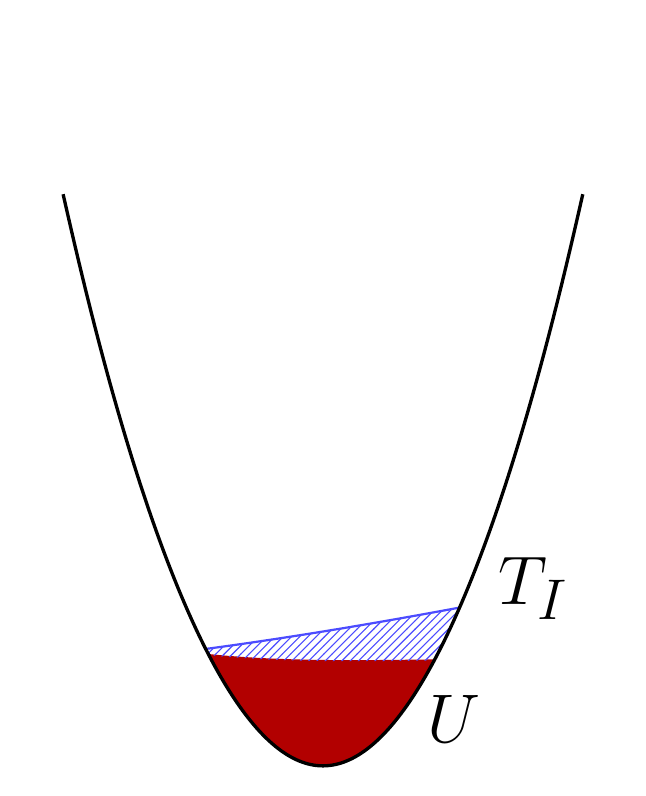
\begin{tikzpicture}[scale=1.5]

    % 1. Definimos o caminho da parábola (representando o conjunto [n] / contêiner)
    % A parábola servirá como "molde" para que as cores não vazem das bordas.
    \def\cupinterior{(-2.5, 6.25) parabola bend (0,0) (2.5, 6.25) -- cycle}

\begin{scope}
        % O comando clip restringe os desenhos subsequentes ao interior da parábola
        \clip \cupinterior;

        % --- Região U (fundo, preenchimento sólido marrom/avermelhado) ---
        \fill[red!70!black] 
            (-3, -1) -- (-3, 1.5) 
            .. controls (-1.0, 0.5) and (1.0, 1.1) .. (3, 0.8) 
            -- (3, -1) -- cycle;
            
        % Linha superior limitante de U
        \draw[red!70!black, thick] 
            (-3, 1.5) .. controls (-1.0, 0.5) and (1.0, 1.1) .. (3, 0.8);

        % --- Região T (meio, hachurada em azul) ---
        \fill[pattern=north east lines, pattern color=blue!70]
            % Borda inferior (acompanha a borda superior de U, da esquerda para a direita)
            (-3, 1.5) .. controls (-1.0, 0.5) and (1.0, 1.1) .. (3, 0.8) 
            % Sobe na borda direita até o final da linha superior de T
            -- (3, 1.7)
            % Borda superior de T (acompanha a linha azul, da direita para a esquerda - nota que os controles estão invertidos)
            .. controls (1.0, 1.3) and (-1.0, 0.9) .. (-3, 0.8) 
            % Fecha o ciclo na borda esquerda descendo até o ponto inicial
            -- cycle;
            
        % Linha superior limitante de T
        \draw[blue!70, thick] 
            (-3, 0.8) .. controls (-1.0, 0.9) and (1.0, 1.3) .. (3, 1.7);
    \end{scope}

    % 2. Desenho do contorno principal externo (a linha preta do "saco")
    % Desenhado por último para ficar por cima das cores
    \draw[very thick] (-2.2, 4.84) parabola bend (0,0) (2.2, 4.84);

    % 3. Rótulos das Regiões (colocados externamente ao lado direito)
    \node[right, font=\Huge] at (0.8, 0.4) {$U$};
    \node[right, font=\Huge] at (1.4, 1.5) {$T_I$};

\end{tikzpicture}

\bigskip

\textbf{Fase I(b)}
Aqui, nosso objetivo é reduzir $A_{\mathrm{I}}$ (tamanho $6\sqrt{n}\log^6 n$) até
$|A| = 6\sqrt{n}\log^2 n$, agora com grau médio menor — e portanto $|T'_{\mathrm{I}}|$ será maior
que $|T_{\mathrm{I}}|$, mas ainda logarítmico.
 Reiniciamos com $A = A_{\mathrm{I}}$ e $T = \emptyset$, mantendo o mesmo $U$.
Aplicamos o algoritmo de contêiner enquanto $|A| \geq 6\sqrt{n}\log^2 n$. Ao final, definimos
$T'_{\mathrm{I}} := T$ e $A'_{\mathrm{I}} := A$.
Enquanto $|A| \geq 6\sqrt{n}\log^2 n$, ainda temos $|A| \cdot |U| \geq 6n$, logo o Lema~\ref{supersaturation1}
continua válido. Porém, agora o grau médio é apenas
\[
  d(H^U(A)) \;\geq\; \frac{|A|\,|U|^2}{6n}
  \;\geq\; \frac{6\sqrt{n}\log^2 n \cdot n/\log^4 n}{6n}
  \;=\; \frac{\sqrt{n}}{\log^2 n} = |U|.
\]
O grau máximo é pelo menos $|U|$, que é menor que na Fase I(a) — por isso o contêiner encolhe
mais devagar e $T'_{\mathrm{I}}$ pode ficar maior.
Cada adição a $T'_{\mathrm{I}}$ remove pelo menos $|U|$ vértices de $A$. Como $A$ começa esta fase
com $|A_{\mathrm{I}}| = 6\sqrt{n}\log^6 n$ vértices, obtemos
\[
  |T'_{\mathrm{I}}| \;\leq\; \frac{|A_{\mathrm{I}}|}{|U|}
  \;=\; \frac{6\sqrt{n}\log^6 n}{\sqrt{n}/\log^2 n}
  \;=\; 6\log^8 n.
\]

\medskip
Assim, ao final da fase I(b), temos $|A'_{\mathrm{I}}| = 6\sqrt{n}\log^2 n$, e $I \subseteq T_{\mathrm{I}} \cup T'_{\mathrm{I}}
\cup A'_{\mathrm{I}}$.


\textbf{[Fase II]}

Ao final das Fases I(a) e I(b), temos $|A'_{\mathrm{I}}| = 6\sqrt{n}\log^2 n$. Se tentássemos
continuar usando o mesmo $U$ (com $|U| = \sqrt{n}/\log^2 n$), o grau médio garantido pelo
Lema~\ref{supersaturation1} seria
\[
  d(H^U(A)) \;\geq\; \frac{|A|\,|U|^2}{6n}
  \;\approx\; \frac{6\sqrt{n}\log^2 n \cdot n/\log^4 n}{6n} = \frac{\sqrt{n}}{\log^2 n} = |U|,
\]
e ao reduzir $|A|$ abaixo de $6\sqrt{n}\log^2 n$, a condição $|A|\cdot|U| \geq 6n$ deixaria de
valer --- o Lema~\ref{supersaturation1} não se aplica mais. A solução é \emph{trocar $U$ por um conjunto maior},
de modo a restaurar a condição de supersaturação. Escolhemos um novo conjunto
\[
  U_{\mathrm{II}} \;\subset\; A'_{\mathrm{I}} \cap I
  \quad \text{com} \quad
  |U_{\mathrm{II}}| = \frac{\sqrt{n}}{\log n}.
\]
Note que $U_{\mathrm{II}}$ é escolhido \emph{dentro} do container $A'_{\mathrm{I}}$ corrente, e
deve ser subconjunto de $I$ para que possamos aplicar a Proposição~\ref{propind} novamente: qualquer
extensão Sidon de $U_{\mathrm{II}}$ é independente em $H^{U_{\mathrm{II}}}(A)$.
Precisamos que $|A| \cdot |U_{\mathrm{II}}| \geq 6n$ enquanto $|A| \geq 6\sqrt{n}\log n$, o que
é satisfeito pois
\[
  6\sqrt{n}\log n \cdot \frac{\sqrt{n}}{\log n} = 6n. \quad \checkmark
\]
O limiar de parada $6\sqrt{n}\log n$ é assim o menor valor de $|A|$ para o qual o Lema~\ref{supersaturation1}
ainda se aplica com este $U_{\mathrm{II}}$.
Fazemos $A \leftarrow A'_{\mathrm{I}} \setminus U_{\mathrm{II}}$ e $T = \emptyset$. Aplicamos o
algoritmo de container no grafo $H^{U_{\mathrm{II}}}(A)$ enquanto $|A| \geq 6\sqrt{n}\log n$.
Ao final, definimos $T_{\mathrm{II}} := T$ e $A_{\mathrm{II}} := A$.
Enquanto $|A| \geq 6\sqrt{n}\log n$, temos $|A|\cdot|U_{\mathrm{II}}| \geq 6n$, portanto
\[
  d(H^{U_{\mathrm{II}}}(A)) \;\geq\; \frac{|A|\,|U_{\mathrm{II}}|^2}{6n}
  \;\geq\; \frac{6\sqrt{n}\log n \cdot n/\log^2 n}{6n}
  \;=\; \frac{\sqrt{n}}{\log n} = |U_{\mathrm{II}}|.
\]
Cada adição a $T_{\mathrm{II}}$ remove pelo menos $|U_{\mathrm{II}}|$ vértices de $A$. Como $A$
começa esta fase com $|A'_{\mathrm{I}}| \leq 6\sqrt{n}\log^2 n$ vértices, obtemos
\[
  |T_{\mathrm{II}}| \;\leq\; \frac{|A'_{\mathrm{I}}|}{|U_{\mathrm{II}}|}
  \;\leq\; \frac{6\sqrt{n}\log^2 n}{\sqrt{n}/\log n}
  \;=\; 6\log^3 n.
\]
Novamente polilogarítmico: o número de escolhas para $T_{\mathrm{II}}$ é $2^{o(\sqrt{n})}$.
Como $U_{\mathrm{II}} \subset A'_{\mathrm{I}}$ e $|A'_{\mathrm{I}}| \leq 6\sqrt{n}\log^2 n$, o
número de escolhas para $U_{\mathrm{II}}$ é
\[
  \binom{6\sqrt{n}\log^2 n}{\sqrt{n}/\log n}
  \;=\; 2^{O(\log\log n)\,\frac{\sqrt{n}}{\log n}},
\]
que é subordem de $2^{O(\sqrt{n})}$ e será absorvido no produto final.

Ao final da fase II, temos $|A_{\mathrm{II}}| < 6\sqrt{n}\log n$, e
\[
  I \;\subseteq\; T_{\mathrm{I}} \cup T'_{\mathrm{I}} \cup U_{\mathrm{II}}
  \cup T_{\mathrm{II}} \cup A_{\mathrm{II}}.
\]


\textbf{[Fases $\mathrm{III}_j$, para $1 \leq j \leq \log\log n$]}

Ao final da Fase II, temos $|A_{\mathrm{II}}| < 6\sqrt{n}\log n$. Gostaríamos de continuar
reduzindo $A$ até que seu tamanho seja $O(\sqrt{n})$ --- pois aí o número de subconjuntos de
$A$ é $2^{O(\sqrt{n})}$, que é a ordem correta. Resta portanto baixar $|A|$ de
$6\sqrt{n}\log n$ até $6\sqrt{n}$, reduzindo por um fator de $2$ a cada fase.

A ideia é a mesma das fases anteriores: cada vez que $|A|$ cai pela metade, dobramos o tamanho
de $U_j$ para manter $|A|\cdot|U_j| \geq 6n$, garantindo que o Lema~\ref{supersaturation1} continue válido.
Como $|A|$ precisa cair por um fator $\log n$ no total (de $\sqrt{n}\log n$ para $\sqrt{n}$),
precisamos de $\log\log n$ fases.

Na $j$-ésima fase, trabalhamos no intervalo
\[
  \frac{6\sqrt{n}\log n}{2^{j-1}} \;>\; |A| \;\geq\; \frac{6\sqrt{n}\log n}{2^j},
\]
e escolhemos
\[
  U_j \;\subset\; A_{j-1} \cap I
  \quad\text{com}\quad
  |U_j| = 2^j\,\frac{\sqrt{n}}{\log n},
\]
onde $A_0 := A_{\mathrm{II}}$ (convenção para $j=1$) e $A_{j-1}$ é o container da fase anterior.

A condição $|A|\cdot|U_j| \geq 6n$ é satisfeita enquanto $|A| \geq 6\sqrt{n}\log n / 2^j$:
\[
  \frac{6\sqrt{n}\log n}{2^j} \cdot 2^j\,\frac{\sqrt{n}}{\log n} \;=\; 6n. \quad \checkmark
\]
Portanto o limiar de parada de cada fase é exatamente o ponto em que a supersaturação deixa de
ser garantida com $U_j$ fixo. Na fase seguinte, dobramos $|U_{j+1}| = 2|U_j|$ e o limiar cai
pela metade, mantendo o produto $|A|\cdot|U_j|$ constante.

Fazemos $A \leftarrow A_{j-1} \setminus U_j$ e $T = \emptyset$. Aplicamos o algoritmo de
container no grafo $H^{U_j}(A)$ enquanto $|A| \geq 6\sqrt{n}\log n / 2^j$. Ao final, definimos
$T_j := T$ e $A_j := A$.

Enquanto $|A| \geq 6\sqrt{n}\log n / 2^j$, temos
\[
  d(H^{U_j}(A)) \;\geq\; \frac{|A|\,|U_j|^2}{6n}
  \;\geq\; \frac{\dfrac{6\sqrt{n}\log n}{2^j}\cdot\dfrac{2^{2j}\,n}{\log^2 n}}{6n}
  \;=\; 2^j\,\frac{\sqrt{n}}{\log n} \;=\; |U_j|.
\]


Cada adição a $T_j$ remove pelo menos $|U_j|$ vértices de $A$. O container de entrada tem
tamanho $|A_{j-1}| < 6\sqrt{n}\log n / 2^{j-1}$, portanto
\[
  |T_j| \;\leq\; \frac{|A_{j-1}|}{|U_j|}
  \;<\; \frac{6\sqrt{n}\log n / 2^{j-1}}{2^j\,\sqrt{n}/\log n}
  \;=\; \frac{6\log^2 n}{2^{2j-1}}
  \;\leq\; 3\log^2 n.
\]
Em particular, $|T_j| = O(\log^2 n)$ para todo $j$, de modo que o número total de escolhas para
$T_1, \ldots, T_{\log\log n}$ é
\[
  \prod_{j=1}^{\log\log n} \binom{n}{3\log^2 n}
  \;=\; 2^{O(\log^2 n \cdot \log\log n \cdot \log\log n)}
  \;=\; 2^{o(\sqrt{n})}.
\]

O número de escolhas para $U_j \subset A_{j-1}$ com $|A_{j-1}| \leq 4\sqrt{n}\log n / 2^{j-1}$
e $|U_j| = 2^j\sqrt{n}/\log n$ é
\[
  \binom{|A_{j-1}|}{|U_j|}
  \;\leq\; \binom{6\sqrt{n}\log n / 2^{j-1}}{2^j\,\sqrt{n}/\log n}.
\]
A Afirmação~\ref{contas} mostra que o produto sobre todas as fases satisfaz
\[
  \prod_{j=1}^{\log\log n}
  \binom{6\sqrt{n}\log n / 2^{j-1}}{2^j\,\sqrt{n}/\log n}
  \;\leq\; 2^{(2\log(12e)+4)\sqrt{n}}
  \;=\; 2^{O(\sqrt{n})},
\]
usando a substituição $x = 6\sqrt{n}\log n / 2^{\log\log n - 1} = 12\sqrt{n}$ e a cota
$\binom{m}{k} \leq (em/k)^k$.

\medskip
Definimos $C := A_{\log\log n}$. Como o limiar de parada da última fase é
\[
  \frac{6\sqrt{n}\log n}{2^{\log\log n}} = \frac{6\sqrt{n}\log n}{\log n} = 6\sqrt{n},
\]
temos $|C| \leq 6\sqrt{n}$. A cobertura acumulada ao longo de todas as fases garante
\[
  I \;\subseteq\; C \;\cup\; T_{\mathrm{I}} \;\cup\; T'_{\mathrm{I}} \;\cup\; T_{\mathrm{II}}
  \;\cup\; \bigcup_{j=1}^{\log\log n} T_j.
\]


\paragraph{Resumo de todas as fases.}
\begin{center}
\renewcommand{\arraystretch}{1.6}
\begin{tabular}{lcccc}
\hline
\textbf{Fase} & \textbf{$U$ usado} & \textbf{$|A|$ ao final} & \textbf{Grau mín.} & \textbf{$|T|$ máximo} \\
\hline
I(a)      & $|U|=\sqrt{n}/\log^2 n$          & $6\sqrt{n}\log^6 n$ & $|U|\log^4 n$ & $\sqrt{n}/\log^2 n$ \\
I(b)      & $|U|=\sqrt{n}/\log^2 n$          & $6\sqrt{n}\log^2 n$ & $|U|$         & $6\log^8 n$ \\
II        & $|U_{\mathrm{II}}|=\sqrt{n}/\log n$ & $6\sqrt{n}\log n$   & $|U_{\mathrm{II}}|$ & $6\log^3 n$ \\
$\mathrm{III}_j$ ($j\geq 1$) & $|U_j|=2^j\sqrt{n}/\log n$ & $6\sqrt{n}\log n/2^j$ & $|U_j|$ & $3\log^2 n$ \\
\hline
\end{tabular}
\end{center}
\bigskip

\subsection*{Contagem final}

\begin{claim}
\label{contas}
\[
  \prod_{j=1}^{\log\log n}
  \binom{6\sqrt{n}\log n / 2^{j-1}}{2^j\,\sqrt{n}/\log n}
  \;\leq\; 2^{(2\log(12e)+4)\sqrt{n}}.
\]
\end{claim}

Precisamos controlar o produto do número de escolhas para $U_1, \ldots, U_{\log\log n}$.
Cada fator $\binom{|A_{j-1}|}{|U_j|}$ conta de quantas formas podemos escolher $U_j$ dentro do
container $A_{j-1}$. O ponto crucial é que, embora cada fator individualmente possa ser grande,
os expoentes formam uma \emph{série geométrica convergente} em $\sqrt{n}$: o fator do passo $j$
contribui com um expoente proporcional a $\sqrt{n}/2^{j-1}$, e a soma
$\sum_{j=0}^\infty 1/2^j = 2$ faz o produto total ser $2^{O(\sqrt{n})}$.

\begin{proof}
Fazemos a substituição $i = j - 1$, de modo que o produto vai de $i = 0$ até
$i = \log\log n - 1$. Para clareza, definimos
\[
  x \;:=\; \frac{6\sqrt{n}\log n}{2^{\log\log n - 1}} \;=\; 12\sqrt{n}.
\]
Este é o tamanho do container na \emph{última} fase (fase $\mathrm{III}_{\log\log n}$), que é o
menor container do processo. Com essa escolha, o tamanho do container na fase $i$ (contando de
trás para frente) é $2^i x$, e o tamanho de $U$ correspondente é $12n / (2^i x) = 12n/(2^i x)$.
Mais precisamente, o $i$-ésimo fator do produto torna-se
\[
  \binom{2^i x}{\;12n/(2^i x)\;},
\]
e o produto original é igual a
\[
  \prod_{i=0}^{\log\log n - 1} \binom{2^i x}{12n / (2^i x)}.
\]

Usamos a desigualdade $\binom{m}{k} \leq \left(\frac{em}{k}\right)^k$, válida para todos
$m \geq k \geq 1$. Com $m = 2^i x$ e $k = 12n/(2^i x)$, obtemos
\[
  \binom{2^i x}{12n/(2^i x)}
  \;\leq\;
  \left(\frac{e \cdot 2^i x \cdot 2^i x}{12n}\right)^{12n/(2^i x)}
  \;=\;
  \left(\frac{e \cdot x^2 \cdot 2^{2i}}{12n}\right)^{12n/(2^i x)}.
\]
Substituindo $x = 12\sqrt{n}$, temos $x^2 = 144n$, logo $ex^2/(12n) = 12e$, e o expoente
$12n/(2^i x) = 12n / (2^i \cdot 12\sqrt{n}) = \sqrt{n}/2^i$. Portanto:
\[
  \left(\frac{e \cdot x^2 \cdot 2^{2i}}{12n}\right)^{12n/(2^i x)}
  \;=\;
  \left(12e \cdot 2^{2i}\right)^{\sqrt{n}/2^i}.
\]

Escrevemos $(12e \cdot 2^{2i})^{\sqrt{n}/2^i}$ como potência de $2$:
\[
  \left(12e \cdot 2^{2i}\right)^{\sqrt{n}/2^i}
  \;=\; 2^{\left[\log(12e) + 2i\right]\cdot \sqrt{n}/2^i}
  \;=\; 2^{\left[(\log(12e) + 2i)\,2^{-i}\right]\sqrt{n}}.
\]

Tomando o produto sobre $i = 0, \ldots, \log\log n - 1$ e usando que todos os termos são
positivos:
\[
  \prod_{i=0}^{\log\log n - 1}
  2^{\left[(\log(12e)+2i)\,2^{-i}\right]\sqrt{n}}
  \;=\;
  2^{\left[\,\sum_{i=0}^{\log\log n-1}(\log(12e)+2i)\,2^{-i}\,\right]\sqrt{n}}
  \;\leq\;
  2^{\left[\,\sum_{i=0}^{\infty}(\log(12e)+2i)\,2^{-i}\,\right]\sqrt{n}}.
\]
Calculamos a série usando as identidades $\sum_{i=0}^\infty 2^{-i} = 2$ e
$\sum_{i=0}^\infty i \cdot 2^{-i} = 2$:
\[
  \sum_{i=0}^{\infty} (\log(12e) + 2i)\,2^{-i}
  \;=\; \log(12e)\sum_{i=0}^\infty 2^{-i} \;+\; 2\sum_{i=0}^\infty i\cdot 2^{-i}
  \;=\; 2\log(12e) + 4.
\]
Portanto:
\[
  \prod_{j=1}^{\log\log n}
  \binom{6\sqrt{n}\log n / 2^{j-1}}{2^j\,\sqrt{n}/\log n}
  \;\leq\; 2^{(2\log(12e)+4)\sqrt{n}}.
  \qquad \blacksquare
\]
\end{proof}

Agora, podemos fazer a contagem final do número de conjuntos de Sidon.
Cada Sidon set $I \subseteq [n]$ é unicamente determinado pelo seu certificado global
\[
  \bigl\{\,U,\, U_{\mathrm{II}},\, U_1, \ldots, U_{\log\log n}\,\bigr\}
  \;\cup\;
  \bigl\{\,T_{\mathrm{I}},\, T'_{\mathrm{I}},\, T_{\mathrm{II}},\,
  T_1, \ldots, T_{\log\log n}\,\bigr\},
\]
e satisfaz $I \subseteq C \cup T_{\mathrm{I}} \cup T'_{\mathrm{I}} \cup T_{\mathrm{II}}
\cup \bigcup_j T_j$, com $|C| \leq 6\sqrt{n}$. O número total de Sidon sets é portanto
majorado pelo produto do número de escolhas de cada componente do certificado.
Organizamos esses fatores na tabela abaixo, mostrando que cada um contribui com um fator
$2^{O(\sqrt{n})}$ ou menor.

\medskip
\begin{center}
\renewcommand{\arraystretch}{1.7}
\begin{tabular}{llll}
\hline
\textbf{Componente} & \textbf{Tamanho máximo} & \textbf{Universo} & \textbf{Nº de escolhas} \\
\hline
$C$ (container final) & $6\sqrt{n}$ & $[n]$ & $2^{|C|} \leq 2^{6\sqrt{n}}$ \\
$U$ & $\sqrt{n}/\log^2 n$ & $[n]$ &
  $\displaystyle\binom{n}{\sqrt{n}/\log^2 n} = 2^{O(\sqrt{n}/\log n)}$ \\
$U_{\mathrm{II}}$ & $\sqrt{n}/\log n$ & $A'_{\mathrm{I}}$, $|A'_{\mathrm{I}}|\leq 6\sqrt{n}\log^2 n$ &
  $2^{O(\log\log n)\,\sqrt{n}/\log n}$ \\
$U_1,\ldots,U_{\log\log n}$ & (varia) & (varia) &
  $2^{(2\log(12e)+4)\sqrt{n}} = 2^{O(\sqrt{n})}$ \;\text{(Afirmação~\ref{contas})} \\
$T_{\mathrm{I}}$ & $\sqrt{n}/\log^2 n$ & $[n]$ & $2^{o(\sqrt{n})}$ \\
$T'_{\mathrm{I}}$ & $6\log^8 n$ & $[n]$ & $2^{o(\sqrt{n})}$ \\
$T_{\mathrm{II}}$ & $6\log^3 n$ & $[n]$ & $2^{o(\sqrt{n})}$ \\
$T_j$ (cada $j$) & $3\log^2 n$ & $[n]$ & $2^{o(\sqrt{n})}$ \\
\hline
\end{tabular}
\end{center}

Multiplicando todos os fatores:
\begin{align*}
S(n)
&\;\leq\;
  \underbrace{2^{|C|}}_{\text{container}}
  \cdot\;
  \underbrace{2^{O(\sqrt{n}/\log n)}}_{U}
  \cdot\;
  \underbrace{2^{o(\sqrt{n})}}_{T_{\mathrm{I}},\,T'_{\mathrm{I}},\,T_{\mathrm{II}},\,T_j}
  \cdot\;
  \underbrace{2^{O(\log\log n)\,\sqrt{n}/\log n}}_{U_{\mathrm{II}}}
  \cdot\;
  \underbrace{\prod_{j=1}^{\log\log n}\binom{|A_{j-1}|}{|U_j|}}_{U_1,\ldots,U_{\log\log n}} \\[6pt]
&\;=\;
  2^{O(\sqrt{n})}
  \cdot\;
  \prod_{j=1}^{\log\log n}
  \binom{6\sqrt{n}\log n/2^{j-1}}{2^j\,\sqrt{n}/\log n} \\[6pt]
&\;\leq\;
  2^{O(\sqrt{n})}
  \cdot\;
  2^{(2\log(12e)+4)\sqrt{n}}
  \;=\; 2^{O(\sqrt{n})},
\end{align*}
onde na segunda linha usamos que $|A_{j-1}| \leq 6\sqrt{n}\log n / 2^{j-1}$, e na terceira
aplicamos o Claim~\ref{contas}. 


\end{proof}

\end{proof}
\section{Prova do limite superior para Sidon \texorpdfstring{$k$}{k}-forte}

Nesta seção, provaremos o limite superior para o número de conjuntos Sidon $k$-fortes em $[n]$,
para todo $k \geq 1$. Para isso, desenvolvemos ferramentas análogas às usadas por Balogh para
conjuntos de Sidon clássicos.

Recordamos que um conjunto $A \subseteq [n]$ é \emph{Sidon $k$-forte} se, para todos
$a_1, a_2, a_3, a_4 \in A$ com $\{a_1, a_2\} \neq \{a_3, a_4\}$, temos
\[
  |a_1 + a_2 - a_3 - a_4| \;\geq\; k.
\]
Em particular, o caso $k = 1$ recupera a definição clássica de conjunto de Sidon.

\medskip
Dado $U \subseteq [n]$ e $A \subseteq [n] \setminus U$, definimos o multigrafo $H_k^U(A)$ com
conjunto de vértices $V(H_k^U(A)) = A$, onde um par $\{a_1, a_2\} \subset A$ forma uma aresta
se, e somente se, existem $u_1, u_2 \in U$ tais que
\[
  |a_1 + u_1 - a_2 - u_2| \;\leq\; k.
\]
A multiplicidade da aresta $\{a_1,a_2\}$ é o número de pares ordenados $(u_1,u_2) \in U\times U$
satisfazendo essa condição. Dizemos que tal par $(u_1,u_2)$ \emph{testemunha} a aresta
$\{a_1,a_2\}$. Note que $H_0^U(A)$ corresponde ao grafo definido por Balogh para conjuntos de
Sidon clássicos, e o caso $k+1$-Sidon forte é tratado por $H_k^U(A)$.

\begin{observation}
Se $A$ é Sidon $k$-forte, então para todos $x,y,z,w \in A$ com $\{x,y\} \neq \{z,w\}$, temos
$|x+y-(z+w)| \geq k$, o que implica que a diferença $x+y-(z+w)$ não pertence ao conjunto
$\{-k+1, \ldots, 0, \ldots, k-1\}$. Em outras palavras, a propriedade Sidon $k$-forte pode ser
lida como uma condição de \emph{evasão}: as diferenças $x+y-(z+w)$ devem evitar uma janela de
$2k-1$ inteiros consecutivos centrada na origem.

Essa perspectiva motiva a definição de $H_k^U(A)$: uma aresta entre $a_1$ e $a_2$ é criada
precisamente quando existe um par $(u_1,u_2) \in U \times U$ tal que a diferença
$(a_1+u_1)-(a_2+u_2)$ cai dentro da janela $\{-k, \ldots, k\}$, isto é,
$|a_1+u_1-(a_2+u_2)| \leq k$. Assim, as arestas de $H_k^U(A)$ marcam os pares de elementos
de $A$ que, juntos com algum par de $U$, violam a condição Sidon $(k+1)$-forte. Um conjunto
independente em $H_k^U(A)$ é, portanto, um conjunto $I \subseteq A$ tal que nenhum par de $I$
admite tal testemunha em $U$; veremos na Proposição~\ref{prop:independente} que isso é
garantido quando $U \cup I$ é Sidon $(k+1)$-forte.
\end{observation}

\begin{proposition}\label{prop:simples}
Se $U \subseteq [n]$ é Sidon $(2k+1)$-forte, então $H_k^U(A)$ é um grafo simples, isto é, toda
aresta tem multiplicidade no máximo $1$.
\end{proposition}

\begin{proof}
Suponha, por contradição, que a aresta $\{a_1, a_2\}$ tem multiplicidade pelo menos $2$. Então
existem dois pares ordenados distintos $(u_1, u_2) \neq (u_3, u_4)$ em $U \times U$, ambos
testemunhando a aresta, isto é,
\[
  |a_1 + u_1 - a_2 - u_2| \;\leq\; k
  \qquad \text{e} \qquad
  |a_1 + u_3 - a_2 - u_4| \;\leq\; k.
\]
Subtraindo as duas expressões e aplicando a desigualdade triangular:
\[
  |u_1 + u_4 - u_2 - u_3|
  \;=\;
  |(a_1 + u_1 - a_2 - u_2) - (a_1 + u_3 - a_2 - u_4)|
  \;\leq\; 2k.
\]
Como $(u_1,u_2) \neq (u_3,u_4)$, temos $\{u_1,u_4\} \neq \{u_2,u_3\}$ (caso contrário
teríamos $u_1=u_3$ e $u_2=u_4$ simultaneamente). Portanto, $u_1,u_2,u_3,u_4 \in U$ formam
uma quádrupla com pares distintos satisfazendo $|u_1+u_4-u_2-u_3| \leq 2k$, o que
contradiz o fato de $U$ ser Sidon $(2k+1)$-forte.
\end{proof}

\begin{proposition}\label{prop:mult2}
Se $U \subseteq [n]$ é Sidon $(2k+2)$-forte, então a multiplicidade de qualquer aresta em
$H_k^U(A)$ é no máximo $2$.
\end{proposition}

\begin{proof}
Suponha, por contradição, que a aresta $\{a_1, a_2\}$ tem multiplicidade pelo menos $3$. Então
existem três pares ordenados distintos $(u_1,u_2)$, $(u_3,u_4)$, $(u_5,u_6) \in U \times U$,
todos testemunhando a aresta. Defina
\[
  d_i \;:=\; (a_1 + u_{2i-1}) - (a_2 + u_{2i}), \qquad i = 1,2,3,
\]
de modo que $|d_i| \leq k$ para todo $i$. Para qualquer par $i \neq j$, calculamos:
\[
  d_i - d_j
  \;=\; (u_{2i-1} + u_{2j}) - (u_{2i} + u_{2j-1}).
\]
Pela desigualdade triangular:
\[
  |(u_{2i-1} + u_{2j}) - (u_{2i} + u_{2j-1})|
  \;=\; |d_i - d_j|
  \;\leq\; |d_i| + |d_j|
  \;\leq\; 2k.
\]
Como $U$ é Sidon $(2k+2)$-forte, para quaisquer $u,u',v,v' \in U$ com $\{u,u'\} \neq \{v,v'\}$
temos $|u+u'-v-v'| \geq 2k+2$. Como $2k+2 > 2k$, a expressão
$(u_{2i-1}+u_{2j})-(u_{2i}+u_{2j-1})$ não pode corresponder a pares distintos; logo
$\{u_{2i-1},u_{2j}\} = \{u_{2i},u_{2j-1}\}$, e portanto $d_i - d_j \in \{-2k, \ldots, 2k\}$
com a restrição adicional de que, se os pares forem distintos, $|d_i-d_j| \geq 2k+2$.
Combinando, $d_i - d_j$ só pode assumir os valores $\{-2k, 2k\}$.

\medskip
Temos portanto três diferenças $d_1-d_2$, $d_1-d_3$, $d_2-d_3$, cada uma em $\{-2k, 2k\}$.
Pelo Princípio da Casa dos Pombos, duas devem ser iguais. Analisamos os casos:

\medskip
\noindent\textbf{Caso 1:} $d_1 - d_2 = d_1 - d_3$. Então $d_2 = d_3$, logo
$d_2 - d_3 = 0 \notin \{-2k, 2k\}$ para $k \geq 1$, uma contradição.

\medskip
\noindent\textbf{Caso 2:} $d_1 - d_2 = d_2 - d_3 = \pm 2k$. Então
$d_1 - d_3 = 2d_2=\pm 4k$, mas $|d_1 - d_3| \leq 2k$, uma contradição para $k \geq 1$.

\medskip
\noindent\textbf{Caso 3:} $d_1 - d_3 = d_2 - d_3$. Então $d_1 = d_2$, e o mesmo argumento
do Caso 1 se aplica.

\medskip
Em todos os casos chegamos a uma contradição. Logo, a multiplicidade de qualquer aresta em
$H_k^U(A)$ é no máximo $2$.
\end{proof}

\begin{proposition}\label{prop:independente}
Sejam $U \subseteq [n]$ um conjunto Sidon $(k+1)$-forte e $I \subseteq A \subseteq [n]
\setminus U$ tais que $U \cup I$ também é Sidon $(k+1)$-forte. Então $I$ é um conjunto
independente em $H_k^U(A)$.
\end{proposition}

\begin{proof}
Suponha, por contradição, que existem $a_1, a_2 \in I$ tais que $\{a_1,a_2\}$ é uma aresta em
$H_k^U(A)$. Por definição, existe um par $(u_1, u_2) \in U \times U$ testemunhando essa aresta,
isto é,
\[
  |a_1 + u_1 - a_2 - u_2| \;\leq\; k.
\]
Como $I \cap U = \emptyset$, os elementos $a_1, a_2 \in I$ e $u_1, u_2 \in U$ são distintos
entre si. Logo a quádrupla $(a_1, u_2, a_2, u_1)$ satisfaz $\{a_1, u_2\} \neq \{a_2, u_1\}$ e
\[
  |a_1 + u_2 - a_2 - u_1|
  \;=\; |a_1 + u_1 - a_2 - u_2|
  \;\leq\; k \;<\; k+1,
\]
contradizendo o fato de $U \cup I$ ser Sidon $(k+1)$-forte.
\end{proof}
\end{document}





%----------------------------------------------------------%


\bibliographystyle{amsplain}
\bibliography{references}

%----------------------------------------------------------%

\end{document}
